\section{Template Method}

A ideia do Template Method é fornecer um esqueleto para um algoritmo 
e deixar para outras classes a tarefa de implementar as funções que 
compõem esse algoritmo. Uma classe abstrata define a operação Template 
Method, onde são executas as etapas do algoritmo, definidas em função 
das operações abstratas ainda não implementadas.

Dessa forma, esse padrão ajuda a evitar repetição de código, concentrando 
em apenas uma classe a estrutura de uma operação. Além disso, 
não só apenas a estrutura do algoritmo como qualquer etapa em 
comum para todas as subclasses pode ser concentrada na superclasse, 
evitando mais ainda a repetição do código. A estrutura do padrão 
pode ser vista na figura \ref{tpmethod_struct}.

\begin{figure}[htb]
	\caption{\label{tpmethod_struct}Estrutura do Template Method}
	\begin{center}
	    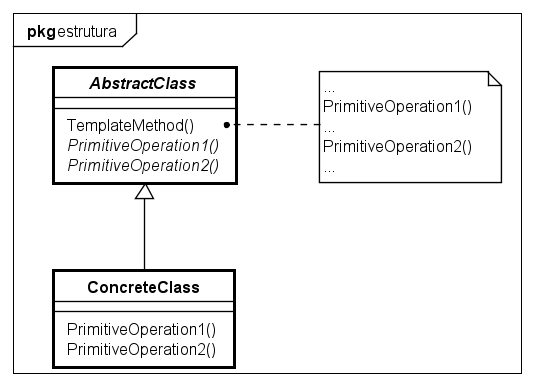
\includegraphics[scale=0.5]{5_padroes-contexto-funcional/5.3_comportamentais/5.3.10_template-method/templatemethod_estrutura.png}
	\end{center}
\end{figure}

\subsection*{Exemplo Orientado a Objetos}

Como exemplo pode ser consideraro um \textit{framework} que fornece uma classe para abrir documentos. Essa classe possui operações abstratas para cada etapada da abertura de um documento, de forma que as subclasses que a estendem podem definir formas diferentes de abrir documentos de tipos diferentes. A operação AddDocument é o template method, responsável por chamar as demais operações implementadas pelas subclasses. 
O diagrama de classes do exemplo pode ser visto na imagem \ref{tpmethod_exemplo}, 
enquanto a implementação pode ser vista no código \ref{ootpmethod}.

\begin{figure}[htb]
	\caption{\label{tpmethod_exemplo}Exemplo de Template Method}
	\begin{center}
	    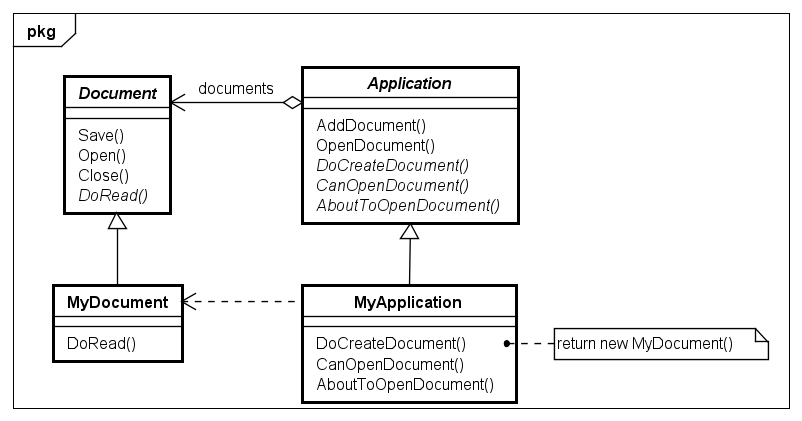
\includegraphics[scale=0.5]{5_padroes-contexto-funcional/5.3_comportamentais/5.3.10_template-method/templatemethod_exemplo.png}
	\end{center}
\end{figure}

\begin{lstlisting}[caption={Template Method Orientação a Objetos},label=ootpmethod]

abstract class Document {
  def Save() : Unit = {
    //Salva um document
  }
  def Open() : Unit = {
    //Abre um documento
  }
  def Close() : Unit = {
    //Fecha um documento
  }
  def DoRead()
}

class MyDocument extends Document {
  def DoRead(): Unit = {
    //Faz leitura do documento
  }
}

abstract class Application {

  var documents : List[Document] = List.empty

  def AddDocument(document : Document) : Unit = {
    documents = document :: documents
  }

  def OpenDocument(fileName : String) : Unit = {
    if(!CanOpenDocument(fileName)){

    } else {
      val doc = DoCreateDocument()
      AddDocument(doc)
      AboutToOpenDocument(doc)
      doc.Open()
      doc.DoRead()
    }
  }

  def DoCreateDocument() : Document
  def CanOpenDocument(fileName : String) : Boolean
  def AboutToOpenDocument(document : Document)
}

class MyApplication extends Application {
  def DoCreateDocument() : Document = new MyDocument
  def CanOpenDocument(fileName : String) : Boolean = {
    //Verifica se documento pode ser aberto
    true
  }
  def AboutToOpenDocument(document : Document): Unit = {
    //Operação ao abrir documento
  }
}

\end{lstlisting}

\subsection*{Contexto Funcional}

No contexto funcional, a mesma ideia pode ser alcançada 
através de funções de alta ordem e composição de funções. 
Nosso método OpenDocument (o \textit{template method}) é 
uma função de alta ordem que recebe como parâmetro todas 
as funções necessárias para executar o algoritmo pré-definido. 
Qualquer função predefinida (como a função AddDocument) é 
chamada de forma comum, exatamente como no exemplo 
orientado a objetos. O exemplo pode ser visto no 
código \ref{fptpmethod}.

\begin{lstlisting}[caption={Template Method Funcional},label=fptpmethod]
    
object Application {

  trait Document {
    def Open()
    def DoRead()
  }

  def AddDocument(document : Document,
                  documents : List[Document]) : List[Document] =
    document :: documents


  def OpenDocument(filename : String,
                   documents : List[Document],
                   DoCreateDocument : () => Document,
                   CanOpenDocument : (String) => Boolean,
                   AboutToOpenDocument : (Document) => Unit) : Unit = {
    if(!CanOpenDocument(filename)){
      //...
    } else {
      var _documents : List[Document] = Nil
      val doc = DoCreateDocument()
      _documents = AddDocument(doc, documents)
      AboutToOpenDocument(doc)
      doc.Open()
      doc.DoRead()
    }
  }

}

\end{lstlisting}

Para definir uma implementação do algoritmo, basta 
definir uma nova função que é a combinação do método 
template com as funções que representam as etapas do 
algoritmo. O código \ref{algotpmethod} define uma 
nova função, MyApplicationOpenDocument, que recebe 
como parâmetro o nome do arquivo e uma lista de 
documentos. Ela retorna a função OpenDocument com as 
funções específicas para o tipo de documento 
desejado sendo passadas como parâmetro, nas linhas 
6, 7 e 8. Dessa forma, a função MyApplicationOpenDocument 
pode ser reutilizada da mesma forma que a classe 
MyApplication seria reutilizada no exemplo orientado 
a objetos.

\begin{lstlisting}[caption={Definição do algoritmo},label=algotpmethod]
    
val MyApplicationOpenDocument = 
    (filename : String, documents : List[Document]) => 
      OpenDocument(filename, documents,
        CreateMyDocument,
        MyCanOpenDocument,
        MyAboutToOpenDocument)

\end{lstlisting}

\subsection*{Vantagens e Desvantagens}

É possível definir novos \textit{templates} com operações 
pré-definidas facilmente criando uma combinação parcial 
das funções necessárias para a execução do algoritmo. 
Assim, poderia ser implementada uma função cujas 
operações DoCreateDocument e CanOpenDocument sejam idênticas, 
mas que permitisse implementações diferentes de 
AboutToOpenDocument. Para que isso pudesse ser feito 
no exemplo orientado a objetos, seria necessário 
definir uma nova subclasse abstrata de Application.

